\chapter{Технологическая часть}

В этом разделе будут выбраны язык программирования для разработки программного обеспечения. 
Также будет представлен интерфейс программы и продемонстрирован ее функционал.

\section{Выбор языка программирования}

Для реализации данной лабораторной работы выбран компилируемый
язык програмирования \texttt{Go}~\cite{golang}. Данный выбор обусловлен следующими причинами:

\begin{itemize}
    \item статическая типизация, помогающая выявлять ошибки на этапе компиляции;
    \item наличие сборщика мусора, который помогает облегчить работу с памятью;
    \item личное желание расширить свои знания в области применения данного языка.
\end{itemize}

\section{Выбор среды разработки}

В качестве среды разработки программного обеспечения был выран Visual Studio Code.
Данный выбор обусловлен следующими причинами: 
\begin{itemize}
    \item предоставляет встроенный отладчик;
    \item наличие опыта работы с данной средой разработки.
\end{itemize}

\section{Интерфейс программного обеспечения}

На рисунке \ref{img:inter} представлен интерфейс программы, который поделен на две части, меню для взаимодействия со сценой и пространство, 
где происходит отрисовка сцены и объектов на ней.

\clearpage
\begin{figure}[h]
    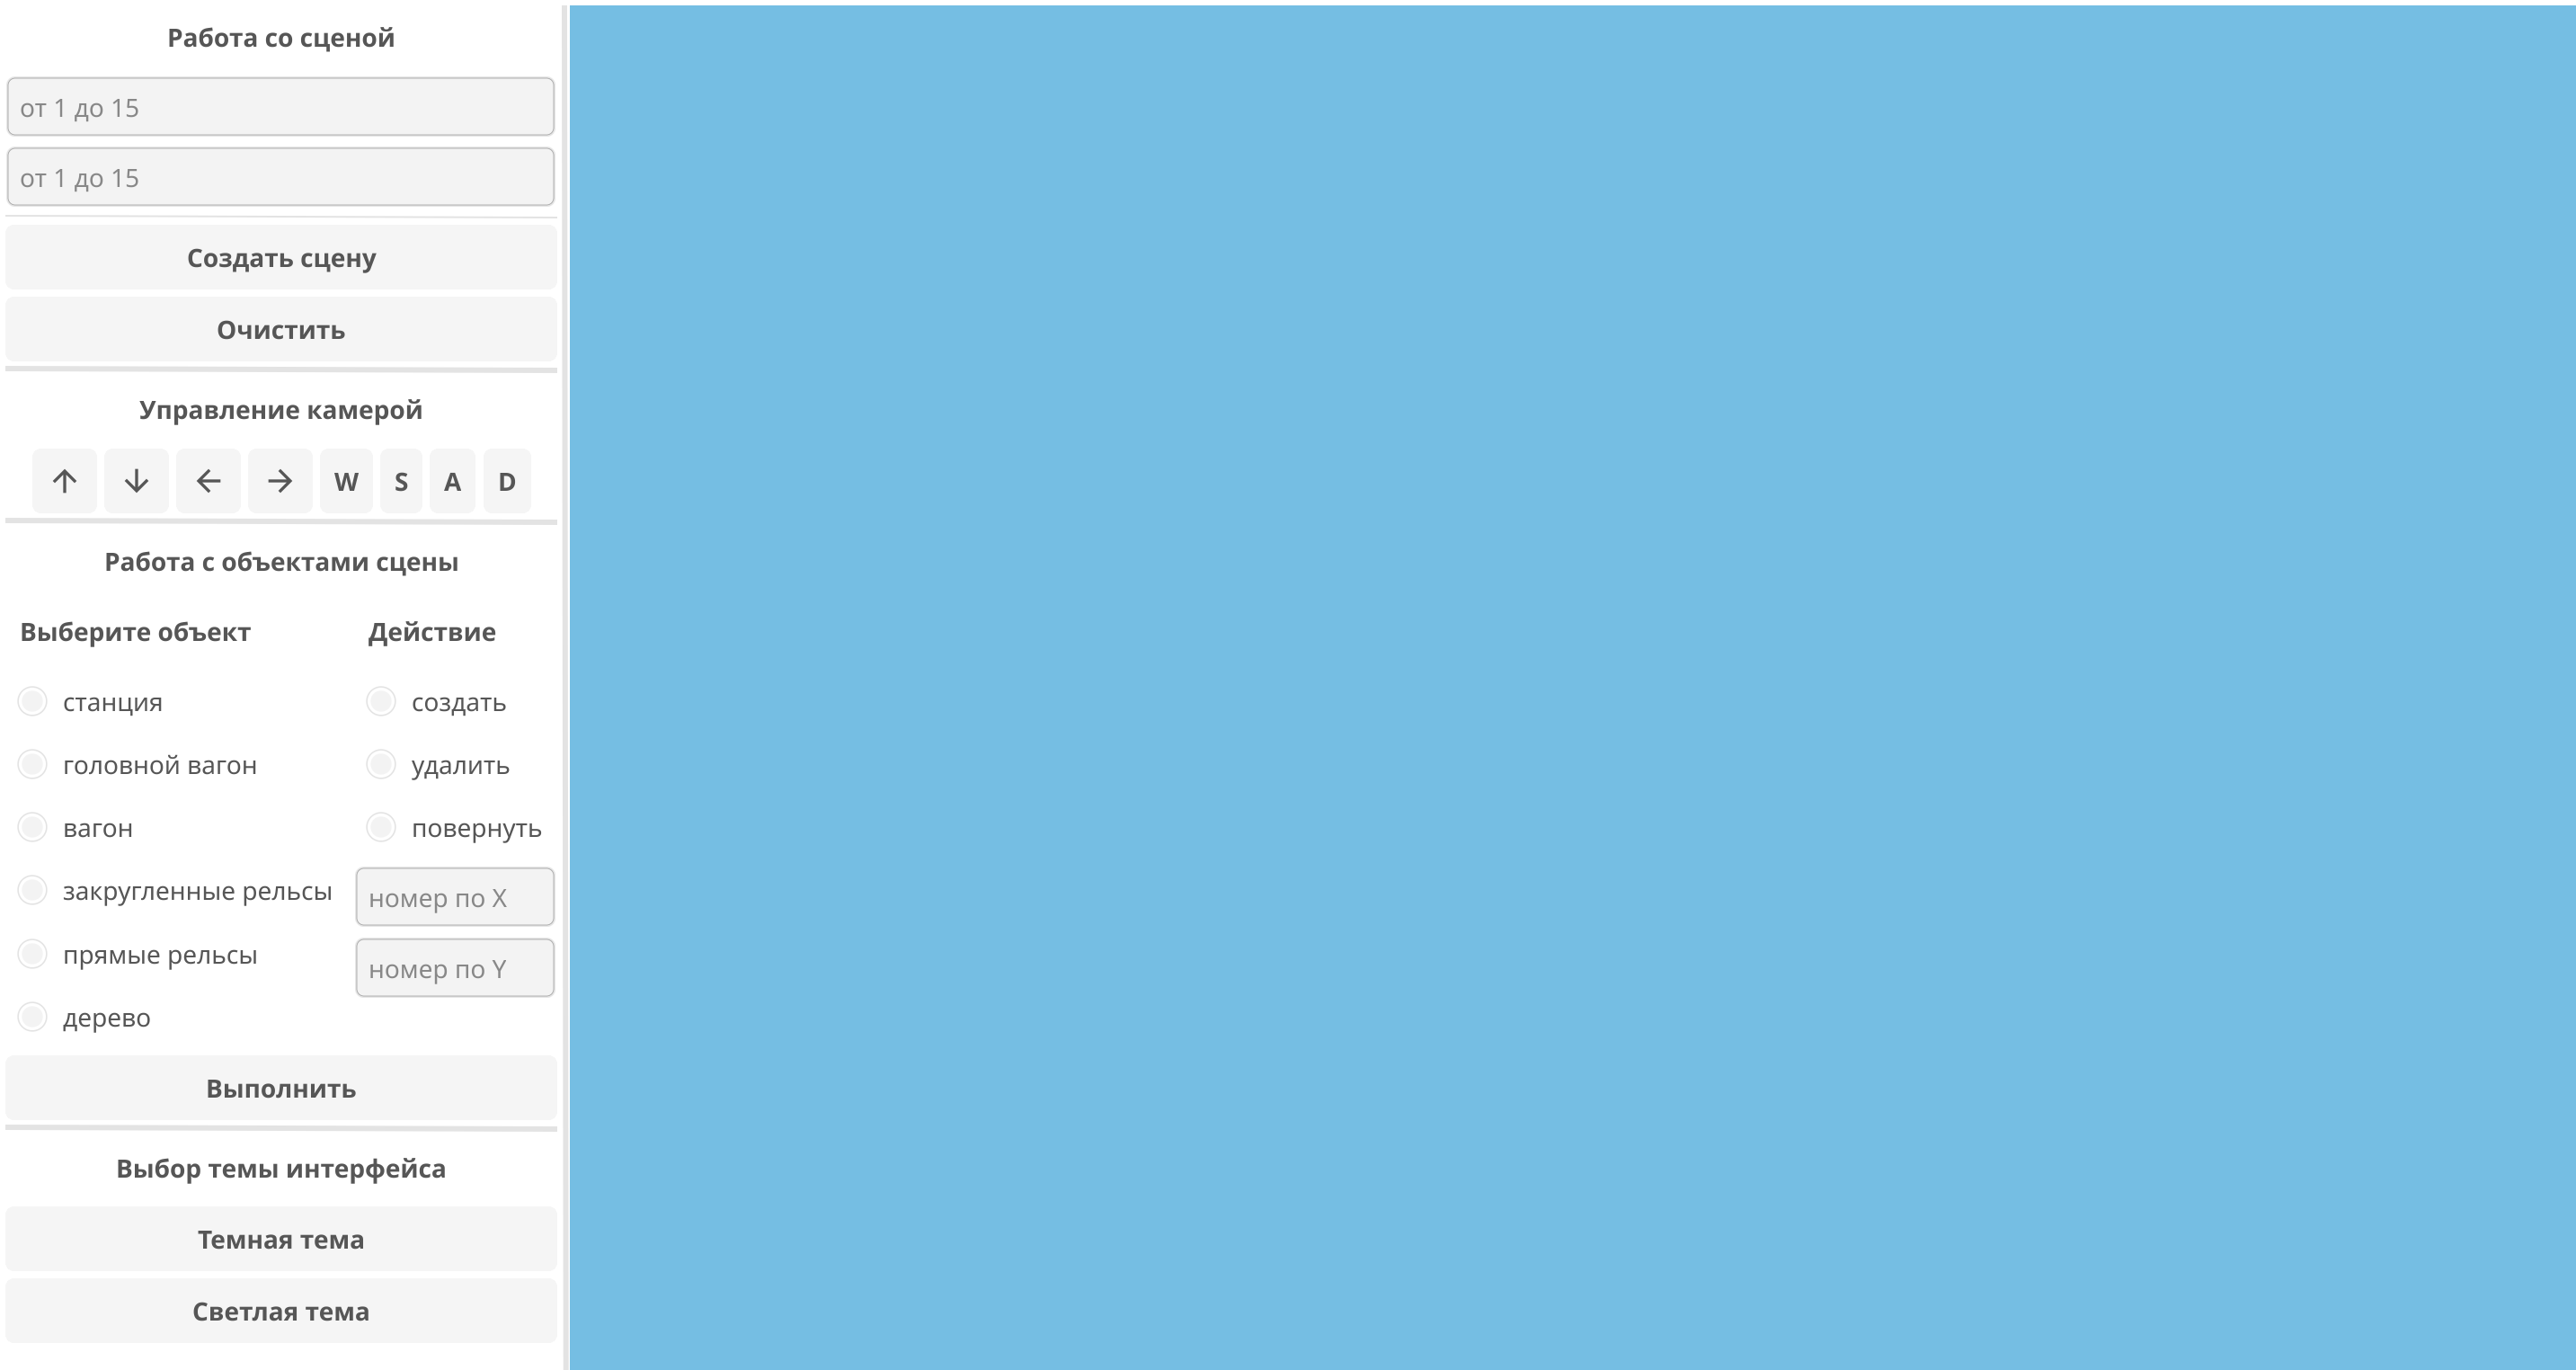
\includegraphics[width=1\linewidth]{img/inter.png}
    \caption{Интерфейс программного обеспечения}
    \label{img:inter}
\end{figure}
\noindent

Меню управления сценой состоит из следующих разделов:
\begin{itemize}
    \item \guillemotleft Работа со сценой\guillemotright-- раздел, отвечающий за создание сцены 
    определенного размера, очистка изображения от сцены и объектов, расположенных на ней;
    \item \guillemotleft Управление камерой\guillemotright -- раздел, предназначенный для управления движением камеры;
    \item \guillemotleft Работа с объектами сцены\guillemotright -- раздел, обеспечивающий создание, удаление и поворот выбранного объекта;
    \item \guillemotleft Выбор темы интерфейса\guillemotright -- раздел, дающий возможность поменять тему программного обеспечения. 
\end{itemize}

Раздел \guillemotleft Работа со сценой\guillemotright предсталвен на рисунке \ref{img:entry}. Данный раздел позволяет 
ввести количество квадратов, из которых будет состоять сцена. Максимальный размер сцены 15x15. Также предоставляется очистка изображения, будет удалена
сцена вместе с объектами, расположенными на ней.

\clearpage
\begin{figure}[h]
    \centering
    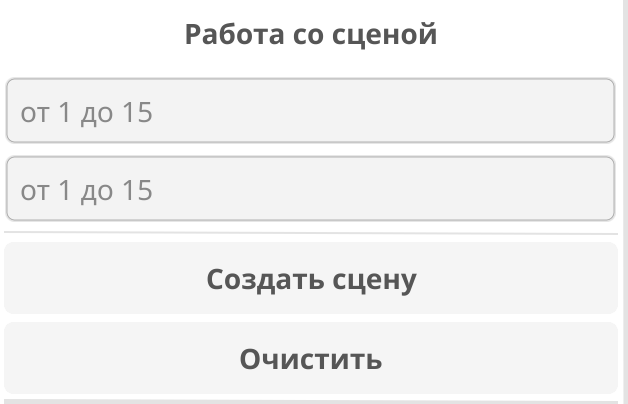
\includegraphics[width=0.5\linewidth]{img/entry.png}
    \caption{Раздел \guillemotleft Работа со сценой\guillemotright}
    \label{img:entry}
\end{figure}
\noindent

Раздел \guillemotleft Управление камерой\guillemotright, предсталвен на рисунке \ref{img:camera}. Данный раздел помогает управлять 
камерой без использования клавиатуры. С помощью стрелок \(\leftarrow\), \(\rightarrow\), \(\uparrow\), \(\downarrow\) осуществляется движение
камеры влево, вправо, вверх и вниз соответсвенно. Кнопки w, s, a, d помогают приближать, отдалять, поворачивать камеру налево и направо.

\begin{figure}[h]
    \centering
    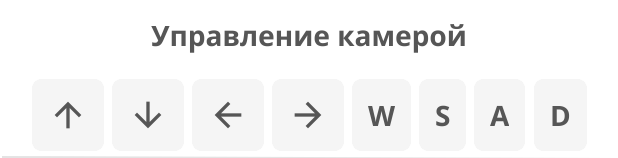
\includegraphics[width=0.8\linewidth]{img/camera.png}
    \caption{\guillemotleft Управление камерой\guillemotright}
    \label{img:camera}
\end{figure}
\noindent

Раздел \guillemotleft Работа с объектами сцены\guillemotright, показанный на рисунке \ref{img:create}, предназначен для создания, поворота и удаления объектов сцены.
Для построения объекта необходимо выбрать объект в подразделе \guillemotleft Выберите объект\guillemotright и 
\guillemotleft создать\guillemotright в подразделе \guillemotleft Действие\guillemotright, далее нужно выбрать ячейку, в которой будет
располагаться объект. Для удаления или поворота объекта необходимо выбрать нужное действие, затем выбрать ячейки, в который располагается
нужный объект.

\clearpage
\begin{figure}[h]
    \centering
    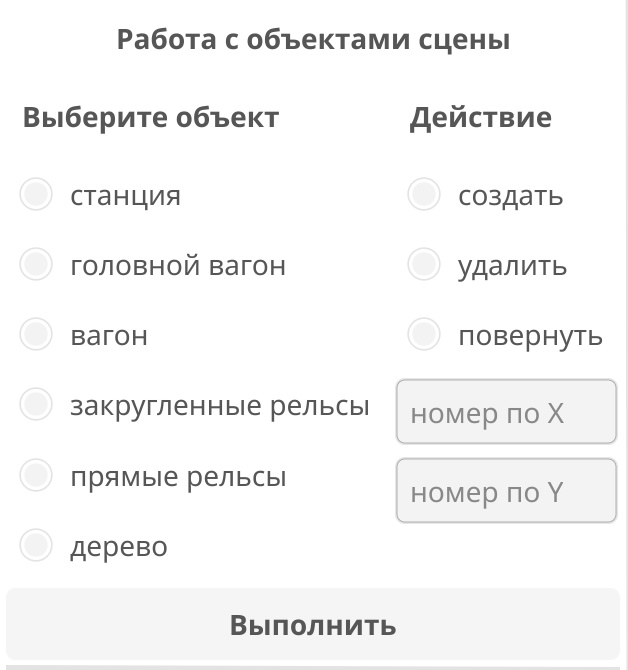
\includegraphics[width=0.65\linewidth]{img/create.png}
    \caption{Раздел \guillemotleft Работа с объектами сцены\guillemotright}
    \label{img:create}
\end{figure}
\noindent

Раздел \guillemotleft Выбор темы интерфейса\guillemotright, представленный на рисунке \ref{img:theme}, позволяет выбрать тему интерфейса.
\begin{figure}[h]
    \centering
    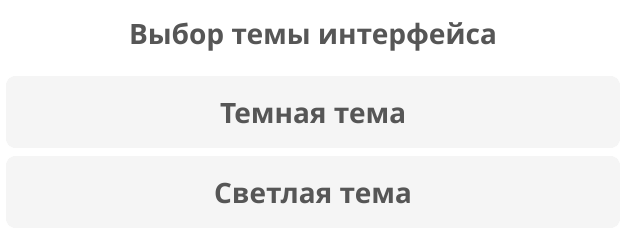
\includegraphics[width=0.7\linewidth]{img/theme.png}
    \caption{Интерфейс программного обеспечения}
    \label{img:theme}
\end{figure}
\noindent

\clearpage
\section{Пример работы программы}

На рисунке \ref{img:exmpl} продемонстирована работа программы при расположении на сцене нескольких объектов.

\begin{figure}[h]
    \centering
    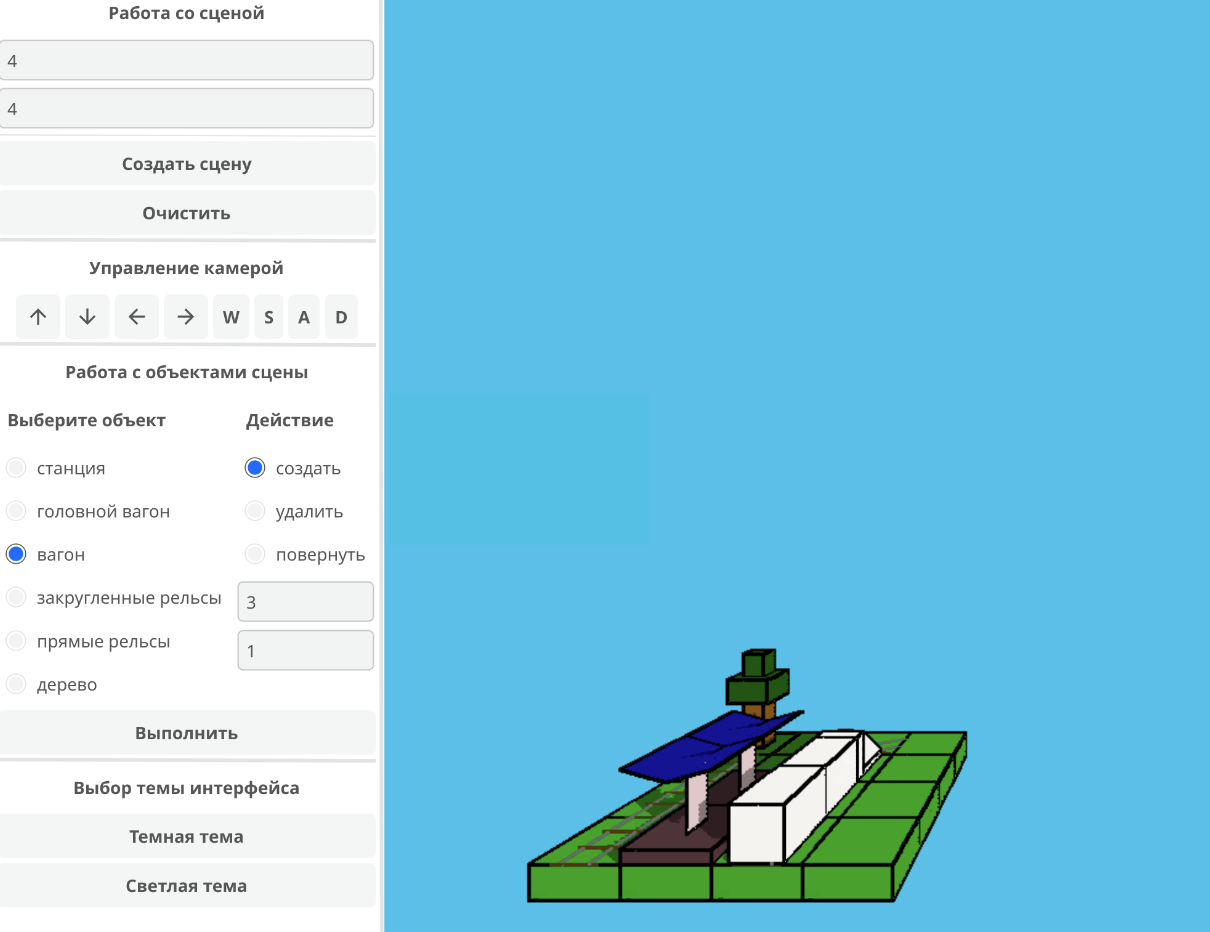
\includegraphics[width=1\linewidth]{img/exmpl.png}
    \caption{Пример работы программного обеспечения}
    \label{img:exmpl}
\end{figure}
\noindent



